% Chapter 3: 16, 27 
% Chapter 4: 20, 35 
% Chapter 5: 10, 26, 30. 
\documentclass{pset}

\providecommand{\Cvx}{\textrm{Conv}}
\providecommand{\Res}{\textrm{Res}}
\renewcommand{\H}{\mathbb{H}}
\providecommand{\ord}{\mathrm{ord}}
\providecommand{\dlog}{\mathrm{dlog}}

\usepackage{multirow}

\title{Math 213a Final}
\author{Lev Kruglyak}
\due{Dec 7, 2023}

\providecommand{\Cvx}{\textrm{Conv}}
\providecommand{\Res}{\textrm{Res}}
\renewcommand{\H}{\mathbb{H}}
\providecommand{\ord}{\mathrm{ord}}
\providecommand{\dlog}{\mathrm{dlog}}



\renewcommand{\abstractname}{Honor Code Statement}
\begin{document}
\maketitle

% \vspace{2.5em}
\begin{abstract}
I affirm my awareness of the standards of the Harvard College Honor Code. While completing this exam, I have not consulted any external sources other than class notes and the textbooks. I have not discussed the problems or solutions of this exam with anyone, and will not discuss them until after the due date.

\medskip
Signed, \underline{\textit{Lev Kruglyak}}.
\end{abstract}
% \vspace{2.5em}

\begin{problem}{3.16}
  Prove that there is no nonconstant analytic function $f : \Delta \to \Delta$ with zeroes at the points $z_n = 1-1/(n+1)$ for $n=1,2,3,\ldots$ %consider f(0)/B_n(0) where B_n(z) is a Blaschke product with zeros at z_1,...,z_n
\end{problem}

\begin{solution}
  Suppose for the sake of contradiction that $f : \Delta \to \Delta$ is some nonconstant analytic function with zeroes at $z_n$. Now consider the Blaschke products: 
  \[
    B_n(z) = \prod_{1\leq k\leq n} \frac{|z_n|}{z_n}\cdot \frac{z_n - z}{1-\overline{z_n} z} = \prod_{1\leq k \leq n} \frac{z_n - z}{1-z_n z}.
  \]
  Since we truncated the zero set to be finite, the zeroes satisfy the Blaschke condition so $B_n$ is an entire function on the disk with zeroes only on the set $\{z_1,\ldots, z_n\}$. In particular, $B_n(0)\neq 0$.

  Now let's consider the functions $f_n(z) = f(z)/B_n(z)$, which must be an analytic function on $\Delta$ since all zeros of $B_n$ are simple and must be zeroes of $f$ as well. We care about the value $f_n(0)= f(0)/B_n(0)$, which we know must finite since $B_n(0)$ is nonzero. 

  We claim that $0<|f_n(0)|\leq 1$. Indeed, if $|f_n(0)|>1$, there would be some region $U$ with $|B_n(z)|>1/|f_n(0)|$ on $\partial U$ and then $|f_n(z)|\leq 1/|B_n(z)| < |f_n(0)|$, which contradicts the maximal principle. Since $|f_n(0)|\leq 1$, we get
  \[
    1\geq |f_n(0)| = \frac{|f(0)|}{|B_n(0)|} \quad\implies\quad |f(0)| \leq |B_n(0)| = \prod_{1\leq k \leq n} \frac{1-1/(n+1)}{1} = \frac{1}{n+1}
  \]
  which proves that $f(0)=0$ since the above inequality holds for any $n$. However, by the Schwarz lemma, the function $|f(z)/z|\leq 1$, so $f(z)/z : \Delta \to \Delta$ has zeroes at $z_n$ as well. This means that it still has a zero at $z=0$ by the same argument, and this proceeds ad infinum. Thus, $f(z)$ has a zero of infinite order, which proves that $f$ is identically zero.
\end{solution}

\begin{problem}{3.27}
  State and prove a necessary and sufficient condition for a meromorphic $1$-form $\omega = \omega(z) \,dz$ on $\C$ to be the logarithmic derivative $\omega =\textrm{dlog}\,f(z)$ of a meromorphic function $f(z)$.
\end{problem}

\begin{solution}
  We claim that there is a one-to-one correspondence:
  \[
    \{ \textrm{dlog}\,f(z)\,dz : f\in \mathcal{M}(\C)\}  \quad\iff\quad \{ \omega(z)\,dz : \omega\in \mathcal{M}(\C), \;\omega\textrm{ has simple poles, integral residues}\}
  \]

  First suppose that $f\in \mathcal{M}(\C)$ is some meromorphic function. We claim that it has simple poles and integral residues. Recall that 
  \[
    \dlog\,f(z) = \frac{f'(z)}{f(z)},
  \]
  so the only poles of $\dlog\, f(z)$ correspond to zeroes or poles of $f(z)$. Notice that if some point $p$ is a zero of $f(z)$ of degree $k$, then it is a zero of $f'(z)$ of degree $k-1$. Thus, $p$ is a simple pole of $\dlog\, f(z)$. Similarly, if $p$ is a pole of $f(z)$ of degree $k$, then it is a pole of $f'(z)$ of degree $k+1$, so again, $p$ is a simple pole of $\dlog\, f(z)$. To see that residues are integral, note that
  \[
    \Res_{p}\, \dlog\,f = \frac{1}{2\pi i}\oint_{S^\epsilon(p)} \frac{f'(z)}{f(z)}\,dz = \#\{\textrm{zeroes of }f(z)\textrm{ in }S^\epsilon(p)\} -\#\{\textrm{poles of }f(z)\textrm{ in }S^\epsilon(p)\}
  \]
  by the argument principle and residue theorem.

  Now suppose conversely that $\omega(z)\in \mathcal{M}(\C)$ is a meromorphic function with simple poles and integral residues, say at $p_k\in \C$ with integral residues. Consider the function $f : \C \setminus \{p_k\} \to \C$ defined in the following way: Pick some point $p\in \C\setminus \{p_k\}$, then for any point $z\in \C\setminus\{p_k\}$ pick a path $\gamma : p \mapsto z$. We then define
  \[
    f(z) = \exp\left(\int_\gamma \omega(z)\,dz\right).
  \]
  First, let's show that this function is well-defined. Suppose $\gamma_1, \gamma_2$ are two paths from $p$ to $z$. Let $C$ be the region encircled by these two paths. By the residue theorem, we have
  \[
    \oint_{\partial C} \omega(z)\,dz = \int_{\gamma_1} \omega(z) \,dz - \int_{\gamma_2} \omega(z)\,dz = 2\pi i \sum_{p_k\in C} \Res_{p_k}(\omega).
  \]
  Since the residues are all integral, this it follows that the integrals $\int_{\gamma_1} \omega(z)\,dz$ and $\int_{\gamma_2} \omega(z)\,dz$ differ by some $2\pi i n$ for $n\in \Z$. This means that after exponentiating, the values of $f(z)$ will be the same. While this function does depend on the initial choice of $p$, changing $p$ would only affect the function up to some constant. This is a common type of construction in complex analysis, and it's clear that it gives us an analytic function on $\C\setminus \{p_k\}$. Finally, taking the logarithmic derivative of $f(z)$, we get
  \[
    \dlog\,f(z) = \frac{f'(z)}{f(z)} = \frac{d}{dz}\int_p^z \omega(z)\,dz\cdot \frac{\exp \left(\int_\gamma \omega(z)\,dz\right)}{\exp \left(\int_\gamma \omega(z)\,dz\right)} = \omega(z).
  \]
  This proves the claim.
\end{solution}

\begin{problem}{4.20}
  Suppose $f\in S$ satisfies $f(iz)=if(z)$. Show that $f(\Delta)$ contains $B(0,1/\sqrt{2})$.
\end{problem}

\begin{solution}
  Suppose $f(z) = z+a_2z^2+z_3z^3+\cdots$. Then the condition $f(iz)=if(z)$ implies that
  \[
    a_k i^k = i a_k \quad \implies \quad a_k(i^{k-1}-1) =0
  \]
  This means that the only nonzero $a_k$ are those with $k\equiv 1\mod 4$. Inspired by the proof of Koebe's 1/4 theorem, let's consider the function $g(z) = f(\sqrt{z})^2$. We can choose some branch cut of the square root such that $g(z)$ can be extended into an analytic function $g : \Delta \to \C$.

  Now we claim that $g\in S$. It's clear from construction that $g(0)=0$, and the derivative has the form
  \[
    \begin{aligned}
      g'(z) = 2f(\sqrt{z}) \cdot f'(\sqrt{z})\cdot \frac{1}{2\sqrt{z}} = \frac{f(\sqrt{z})f'(\sqrt{z})}{\sqrt{z}} 
      &= \frac{(z^{1/2}+ a_5z^{5/2}+\cdots) (1+5a_5z^2+9a_9z^4\cdots)}{\sqrt{z}}\\
      &= (1+a_5 z^2+a_9 z^4+\cdots)(1+5a_5z^2+9a_9z^4+\cdots)\\
      &= 1 + 6a_5z^2 + \cdots
    \end{aligned}
  \]
  This means that $g'(0)=1$, so $g$ is a univalent map. Following the proof of Koebe's theorem, let's suppose $p\not\in f(\Delta)$. This means that $p^2\not\in g(\Delta)$ since $\sqrt{\Delta} = \Delta$. By the argument in the proof, we conclude that
  \[
    |1/p^2| - 2 \leq |6a_5 + \frac{1}{p^2}| \leq 2 \quad\implies\quad |p|\geq 1/\sqrt{2}.
  \]
  This proves that $B(0,1/\sqrt{2})\subset f(\Delta)$.

\end{solution}

\begin{problem}{4.35}
  Let $f(z)$ be an entire nonzero function such that $f(z)$ is never zero and $f^{-1}(1)$ is finite. Prove that $f$ is constant.
\end{problem}

\begin{solution}
  Since $f$ is never zero, it is a function $f : \C \to \C^*$. We can thus lift to the universal cover $\C$ to get a map $F : \C \to \C$, with $f = \exp(F)$. Now since $f^{-1}(1)$ is finite, it follows that $F^{-1}(2\pi i \Z)$ must be finite as well. This means that $F$ omits infinitely many values, so it is constant by Picard's little theorem. This proves that $f$ is constant.
\end{solution}

\begin{problem}{5.10}
  Where are the 9 flexes of the cubic curve $V\subset \CP^2$ defined by $x^3+y^3=1$? How many of these are real?
\end{problem}

\begin{solution}
  Let's begin by considered a homogenized form of these equations, say $f(x,y,z) = x^3+y^3+z^3$, which has a well-defined zero locus in $\CP^2$. The Hessian determinant of this curve is 
  \[
    H(x,y,z) = \begin{vmatrix} 6x & 0 & 0 \\ 0 & 6y & 0 \\ 0 & 0 & 6z\end{vmatrix} = 216xyz,
  \]
  so at any flex of the curve, we would have $xyz=0$. Assuming without loss of generality that $z=0$, we thus have the equation $x^3 = -y^3$, so scaling $y=-1$ we get $x^3-1=0$ and so $x$ is a 3rd root of unity. Thus, the $9$ flexes are:
  \[
  \begin{aligned}
    [1: -1: 0] &\quad &[1: 0: -1]&\quad &[0: 1: -1] \\
    [\omega: -1: 0] &\quad &[\omega: 0: -1]&\quad &[\omega: 1: -1] \\
    [\omega^2: -1: 0] &\quad &[\omega^2: 0: -1]&\quad &[\omega^2: 1: -1] \\
  \end{aligned}
  \]
  where $\omega$ is a primitive 3rd root of unity. The real flexes correspond to the points $(1,0)$, $(0,1)$, and $\infty$. The first two of these are the classical inflection points of the real curve $x^3 + y^3 -1$.
\end{solution}

\begin{problem}{5.26}
  Let $L$ be the length in the hyperbolic metric of the closed geodesic $\gamma$ on $X=\widehat{\C} - \{0,1,\infty\}$ that makes a figure $8$ around $0$ and $1$. Show that $L= \log(17+12\sqrt{2})$. %show that gamma corresponds to a matrix of trace 6 in pi_1(X)=Gamma(2)
\end{problem}

\begin{solution}
  Recall that the hyperbolic metric on $X$ is induced as the descent of the hyperbolic metric on $\H$ under the quotient map $\lambda : \H \to X$ by the action of the group $\Gamma(2)$. Thus, we can lift the figure 8 geodesic to the upper half plane, which we mark with some unit hyperbolic geodesics:
  \[
  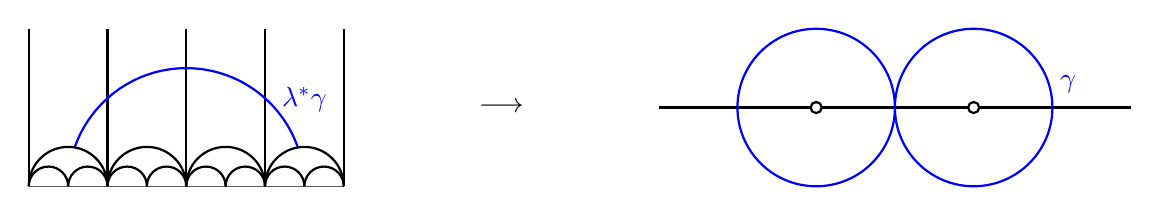
\begin{tikzpicture}
  \begin{scope}[xshift = 0, yshift=0]
    % Draw vertical lines at x = -1, 0, 1, 2, 3
    \foreach \x in {-1,0,1,2,3} {
      \draw[thick, black] (\x,0) -- (\x,2);
    }

      \draw[thick, black] (-1,0) -- (3,0);

      \node[blue] at (2.5,1.1) {$\lambda^*\gamma$};
    \draw[thick, blue] (2.5,0) arc (0:180:1.5);

    % Draw semicircular arcs between each pair of vertical lines
    \foreach \x in {-1,0,1,2} {
      % Calculate radius of the semicircle
      \pgfmathsetmacro{\radius}{(\x+1-\x)/2}
      \pgfmathsetmacro{\radiuss}{(\x+1-\x)/4}
      % Draw the arc
      \fill[white] (\x+\radius+1/2,0) arc (0:180:\radius);
      \draw[thick, black] (\x+\radius+1/2,0) arc (0:180:\radius);
      \draw[thick, black] (\x+\radius+1/2,0) arc (0:180:\radiuss);
      \draw[thick, black] (\x+\radius,0) arc (0:180:\radiuss);
    }
  \end{scope}

  \begin{scope}[xshift = 10cm, yshift=0]
      \node at (-5,1) {$\longrightarrow$};
      \draw[thick, black] (-3,1) -- (3,1);

      \draw[thick, blue] (1,1) circle (1);
      \draw[thick, blue] (-1,1) circle (1);

      \node[blue] at (2.2,1.3) {$\gamma$};
      \draw[thick, black, fill=white] (1,1) circle (2pt);
      \draw[thick, black, fill=white] (-1,1) circle (2pt);
  \end{scope}
  \end{tikzpicture}
  \]
  The hyperbolic length of the geodesic $\gamma$ is then the length of $\lambda^*\gamma$ in the hyperbolic metric on $\H$. Working in polar coordinates, let $\alpha$ be the angle to the start of the arc, which has radius $\sqrt{2}$. The length is then
  \[
    L = \int_{\lambda^* \gamma} \frac{dz}{\textrm{Im}(\lambda^* \gamma)} = \int_\alpha^{\pi - \alpha} \frac{d\theta}{\sin(\theta)} = \log(\cot^2(\alpha/2)).
  \]
  To calculate $\cot(\alpha/2)$, we notice that it is an angle in a right triangle with side lengths $\sqrt{2}, 1/2$, and hypotenuse $3/2$. This means that $\sin(\alpha) = 1/3$ and $\cos(\alpha)=2\sqrt{2}/3$. By the half angle formula, we can then evaluate $\cot(\alpha/2) = \sin(\alpha)/(1-\cos(\alpha))  = 3+2\sqrt{2}.$ This means that $L=\log (3+2\sqrt{2})^2 = \log(17+12\sqrt{2})$.
\end{solution}

\begin{problem}{5.30}
  Prove that $\lambda(i/2) = 12\sqrt{2}-16$.
  % hint lettting X_tau = C/Z + tZ, lambda(t) is the cross ration of critical values of any degree two map f_tau : X_tau \to \widehat{C}. for the square torus, choose f_i so tha its critical values are roots of unity f_{i/2}(z) = f_i(z) + f_i(z)^{-1})^-1/2 and find that its critical values are {-1, -1\sqrt{1/2}, sqrt{1/2}, 1}
\end{problem}

\begin{solution}
  We'll follow the procedure laid out in the hint, so let $\wp$ be the Weierstrass function for the Gaussian integer lattice $\Z[i]$. To calculate its critical values, recall that the cubic for the curve is $4x^3-g_2x = 4x(x-\sqrt{g_2}/2)(x+\sqrt{g_2}/2)$, so $e_0 = \infty, e_1=\sqrt{g_2}/2, e_2=-\sqrt{g_2}/2, e_3=0$. We would like to compose with some transformation which sends these critical values to solutions of $x^4+1=0$.

  First, we scale $\wp$ to be $(2/\sqrt{g_2}) \wp$ so that the critical values are $e_0=\infty, e_1=1, e_2 = -1, e_3=0$. Let's find some M\"obius transformation which sends $\infty \mapsto i, 1 \mapsto 1, -1\mapsto -1, 0 \mapsto -i$. This transformation is given by $(z-i)/(1-iz)$. Now if we multiply this function $\zeta = e^{\pi i /4}$, these points are sent to $i\zeta, \zeta, -\zeta, -i\zeta$, which are exactly the solutions to $x^4+1=0$. Let's call this function
  \[
    A(z) =\zeta\frac{z-i}{1-iz}.
  \]
  Composing with the previous function, we get $f_i(z) = A((2/\sqrt{g_2}) \wp(z))$, a periodic function $X_i \to \widehat{\C}$. Motivated by the hint, we can see that properties of $\wp$ such as the addition formula and corresponding differential equations give us the identity
  \[
    f_i(z+i/2) = \frac{1}{f_i(z)},
  \]
  so let's set $f_{i/2}(z) = (f_{i}(z) - f_{i}^{-1}(z))/2$. By the preceding remarks, this is a function $X_{i/2} \to \widehat{\C}$ with critical values:
  \[
    \pm\frac{i\zeta + 1/i\zeta}{2} = \pm\frac{i\zeta + \zeta}{2} = \pm\frac{1}{\sqrt{2}},\quad \pm \frac{1+1/1}{2} = \pm 1
  \]
  We thus have a function $f_{i/2} : X_{i/2} \to \widehat{\C}$ with critical values $\{-1, -1/\sqrt{2}, 1/\sqrt{2}, 1\}$. Computing the cross ratio gives us the desired value:
  \[
    \lambda(i/2) = \frac{(e_1 - e_0)(e_3-e_2)}{(e_3 - e_0)(e_1 - e_2)} =\frac{(-1/\sqrt{2} + 1)(1/\sqrt{2}+1/\sqrt{2})}{(1/\sqrt{2}+1)(-1/\sqrt{2}-1/\sqrt{2})}= 12\sqrt{2}-16
  \]
\end{solution}

\end{document}
